\subsection*{ Префиксные суммы, сортировка событий, метод двух указателей [8]}
\begin{center}
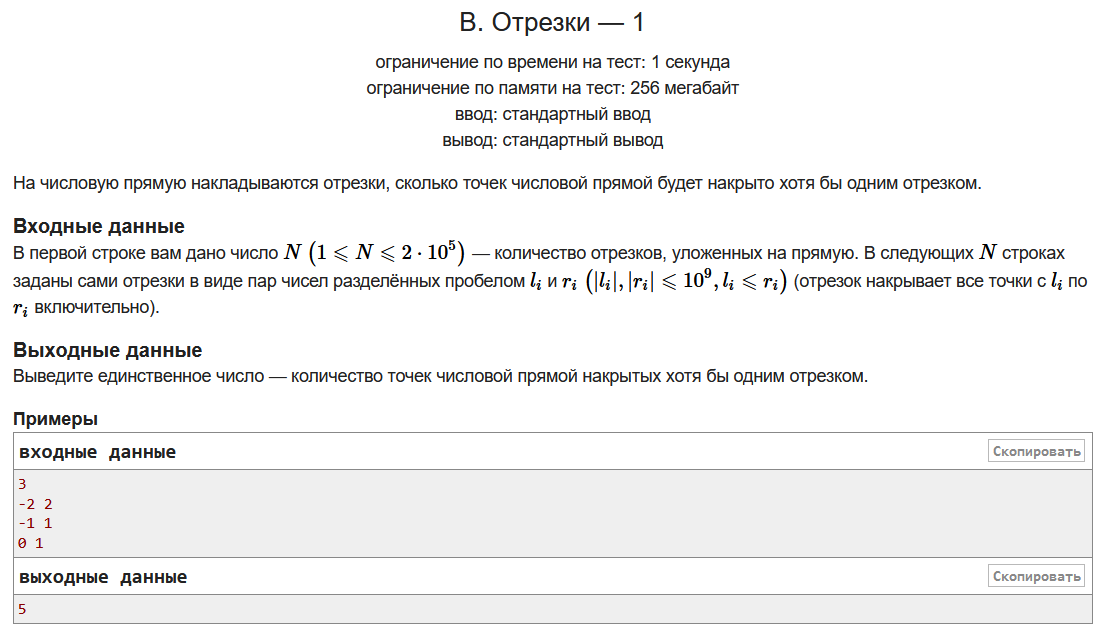
\includegraphics[width=\textwidth]{10B.png}
\end{center}
\subsubsection*{Идея решения}
Реализуем метод сканирующей прямой: создадим массив, в котором каждом элементе будет храниться два числа - первое число координата точки, второе число приоритет точки(0 - открывающая точка, 1 - закрывающая точка). К тому же будем хранить две переменные $ans$ и $q$, которые будут отвечать за кол-во точек не накрытых хотя бы одним отрезком и кол-во "открытых" отрезков. Далее будем обрабатывать сами отрезки: если текущая точка  открывающая, то добавим единицу к переменной $q$ и проверим равенство $q = 1$, если равенство справделиво, то добавим к переменной $ans$ разницу между текущей точкой и предыдущей, если точка закрывающая, то вычтем из $q$ единицу. Ответ равен $last - first - ans +1$, где $last$ - координата крайней правой точки, $first$ - координата крайней левой точки. Асимптотика $O(n\log{}n)$.
\subsubsection*{Исходный код}
\begin{lstlisting}
#include <iostream>
#include <cmath>
#include <algorithm>
#include <vector>
#include <iomanip>
#include <unordered_map>
#include <unordered_set>
#include <map>
#include <set>
#include <string>
#include <stack>
#include <deque>

using namespace std;
typedef long long ll;

int main() {
    ios_base::sync_with_stdio(false);
    cin.tie(0);
    cout.tie(0);
    ll n;
    cin >> n;
    vector<pair<ll, ll>> a(2*n);
    for (int i = 0; i < 2*n; i+=2) {
        ll l, r;
        cin >> l >> r;
        a[i] = { l, 0 };
        a[i + 1] = { r,1 };
    }
    sort(a.begin(), a.end());
    ll ans = 0;
    ll q = 0;
    for (int i = 0; i < 2 * n; i++) {
        if (a[i].second == 0) {
            ++q;
            if (q == 1 and i) {
                ans += a[i].first - a[i - 1].first - 1;
            }
        }
        else {
            --q;
        }
    }
    cout << a[2 * n - 1].first - a[0].first - ans + 1;
    return 0;
}
\end{lstlisting}
\subsubsection*{Фрагмент турнирной таблицы контеста}
\begin{center}
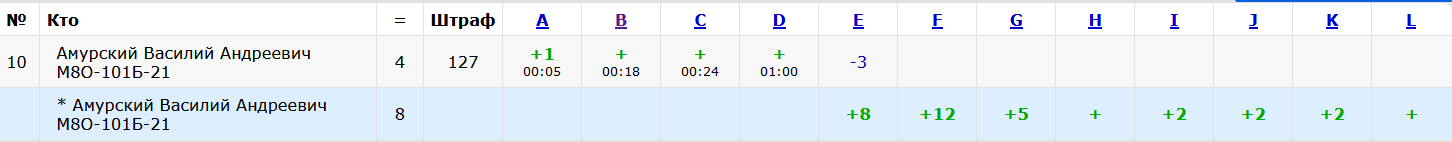
\includegraphics[width=\textwidth]{state10.png}\newline\noindent
\end{center}

\subsubsection*{Выводы}
Задача решена, проблем не возникло.
